\documentclass[aspectratio=169]{beamer}

\usetheme{default}
\usepackage[utf8]{inputenc}
\usepackage[brazil]{babel}
\usepackage{tikz}
\usepackage{tabularx}
\usepackage{amsmath}
\usepackage{booktabs}
\usepackage{multirow}
\usepackage{graphicx}
\usepackage{hyperref}
\usepackage{amssymb}
\usepackage{colortbl}

% logos em presentation/imgs; figuras desta apresentação em ./figuras
\graphicspath{{../}{figuras/}}

\setbeamertemplate{footline}[frame number]
\setbeamertemplate{frametitle}[default][center]

\mode<presentation>{
\usetheme{Dresden}
\usecolortheme{seagull}
}

\setbeamertemplate{headline}{}

\definecolor{peeblue}{RGB}{1,123,165}
\definecolor{darkblue}{RGB}{0,65,115}

\setbeamercolor*{palette primary}{fg=black,bg=peeblue!80}
\setbeamercolor*{palette secondary}{fg=black,bg=peeblue!80!gray!80}
\setbeamercolor*{palette tertiary}{fg=black,bg=peeblue!100}
\setbeamercolor*{palette quaternary}{fg=black,bg=peeblue!110}

\usebackgroundtemplate
{%
    \begin{picture}(210,40)(-5,2)
    
\includegraphics[width=0.07\paperwidth,keepaspectratio]{imgs/pee-logo-short.png}
    \end{picture}%
}

\title{Reconhecimento Acústico de Alvos Submarinos no Dataset IARA}
\subtitle{DEMON e Augmentation com Fundo de Mar Agitado}
\author{Evandro Rocha}
\date{Novembro de 2026}

\institute
{
  Universidade Federal do Rio de Janeiro\\
  UFRJ / COPPE / PEE
}

\newcommand{\cahi}[1]{\cellcolor{green!30}\textbf{#1}}
\newcommand{\calo}[1]{\cellcolor{red!20}#1}
\newcommand{\camd}[1]{\cellcolor{yellow!35}#1}

\begin{document}

{
\usebackgroundtemplate{
    \begin{picture}(210,55)(-5,0)
    
\includegraphics[height=0.14\paperwidth,keepaspectratio]{imgs/pee-logo.png}
    \end{picture}%
    \begin{picture}(210,55)(-28,2)
    
\includegraphics[height=0.14\paperwidth,keepaspectratio]{imgs/coppe-logo.pdf}
    \end{picture}
}
\begin{frame}
  \bigskip\bigskip\bigskip\bigskip
  \titlepage
\end{frame}
}

\begin{frame}{Agenda da Apresentação}
  \footnotesize
  \setbeamercolor{block title}{bg=darkblue,fg=white}
  \setbeamercolor{block body}{bg=peeblue!8,fg=black}
  \setbeamertemplate{section in toc}{%
    \vspace{0.14cm}%
    \leavevmode%
    \tikz[baseline=-0.65ex]\node[circle,fill=peeblue,text=white,inner sep=0pt,font=\tiny\bfseries,minimum size=1.35em]{\inserttocsectionnumber};%
    \hspace{0.35em}%
    \inserttocsection\par%
  }
  \begin{columns}[t]
      \begin{column}{0.6\textwidth}
          \begin{block}{\small\textbf{DEMON e Mar Agitado}}
              \tableofcontents
          \end{block}
      \end{column}
  \end{columns}
\end{frame}

\begin{frame}{Resumo}
    \footnotesize
    \begin{block}{\small Pergunta: o DEMON aproveita o augmentation dos LARGE com fundo de mar agitado?}
        \scriptsize
        \begin{enumerate}
            \setlength{\itemsep}{3pt}
            \item \textbf{Motivação:} no LOFAR, misturar ruído de mar agitado não ajudou, porque o ruído apagava o grave do LARGE. O DEMON mede \emph{ritmos} de modulação (eixo, pás) na banda de 1--2 kHz, onde o ruído de mar mais cresce.
            \item \textbf{O DEMON sozinho é mais fraco que o LOFAR:} SP 45,7 contra 56,1 (mesma MLP, split por navio).
            \item \textbf{O augmentation também não ajuda no DEMON:} recall de LARGE 60,8 $\rightarrow$ 56,2\% (não significativo).
            \item \textbf{Mesmo mecanismo do LOFAR:} o ruído deixa as linhas de modulação mais rasas; com muito ruído, 61\% das cópias de LARGE ficam com o contraste de um navio $<$ 100 m.
        \end{enumerate}
    \end{block}
    \vspace{0.1cm}
    {\tiny Experimento separado dos de LOFAR. Notebook: \texttt{notebooks/42\_demon\_augmentation\_mar.ipynb}.\par}
\end{frame}

%===========================================
\section{O Que É o DEMON}

\begin{frame}
    \centering
    \huge O Que É o DEMON
\end{frame}

\begin{frame}{DEMON: Os Ritmos do Hélice}
    \footnotesize
    \begin{columns}[t]
        \column{0.5\textwidth}
        \begin{block}{\small Como é calculado}
            \scriptsize
            \begin{enumerate}
                \setlength{\itemsep}{2pt}
                \item Filtra o áudio em \textbf{1--2 kHz} (ruído de cavitação).
                \item Tira o \textbf{envelope} (retificação).
                \item Reduz para 50 Hz e calcula o espectro do envelope.
                \item Picos em poucos Hz = \textbf{rotação do eixo} e \textbf{passagem das pás}.
            \end{enumerate}
            Janela de 10,24 s a cada 5,12 s; 253 frequências de 0,4 a 25 Hz.
        \end{block}
        \column{0.46\textwidth}
        \begin{block}{\small Contraste (pico / mediana do DEMON)}
            \scriptsize
            \centering
            \begin{tabular}{lc}
            \toprule
            Classe & Contraste (mediana) \\
            \midrule
            SMALL & 9,4 dB \\
            MEDIUM & 9,7 dB \\
            LARGE & \cahi{12,0 dB} \\
            BACKGROUND & 3,9 dB \\
            \bottomrule
            \end{tabular}

            \vspace{0.1cm}
            Os LARGE têm as linhas de modulação mais marcadas; sem navio, o envelope do ruído não tem ritmo.
        \end{block}
    \end{columns}
\end{frame}

\begin{frame}{DEMON Médio por Classe}
    \centering
    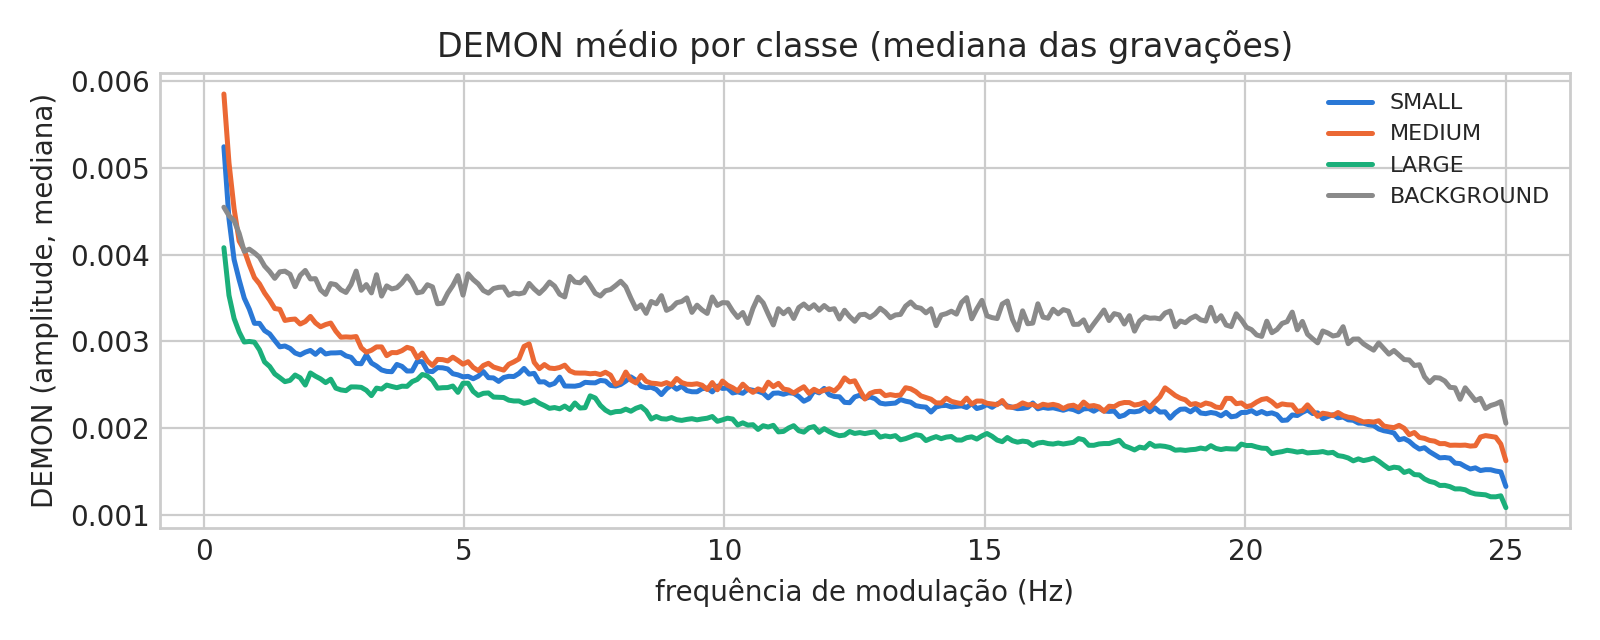
\includegraphics[width=0.82\textwidth]{demon_classes.png}

    \vspace{0.05cm}
    \begin{alertblock}{Leitura}
        \scriptsize
        Na mediana das gravações as linhas se apagam (cada navio tem as suas, em frequências diferentes). O que sobra é o nível: o BACKGROUND, sem ritmo, fica com o espectro mais ``cheio'' e plano.
    \end{alertblock}
\end{frame}

\begin{frame}{Referência: DEMON $\times$ LOFAR na Mesma MLP}
    \footnotesize
    \begin{table}
    \centering
    \scriptsize
    \setlength{\tabcolsep}{4pt}
    \begin{tabular}{llcccccc}
    \toprule
    Representação & Split & SP & ACC & SMALL & MEDIUM & LARGE & BACKGROUND \\
    \midrule
    LOFAR & por navio & \cahi{56,1} & 58,3 & 49,8 & 34,5 & 67,7 & 81,1 \\
    DEMON & por navio & \calo{45,7} & 49,4 & \calo{28,2} & 32,4 & 60,8 & 76,3 \\
    \midrule
    LOFAR & por gravação & 67,4 & 67,8 & 54,1 & 65,9 & 71,2 & 80,0 \\
    DEMON & por gravação & 52,8 & 54,3 & 33,8 & 46,3 & 65,1 & 72,2 \\
    \bottomrule
    \end{tabular}
    \end{table}
    {\tiny MLP h32-16 do NB29, 4 classes, mesmos folds, sem augmentation; média de 10 folds; previsão por gravação = voto das janelas.\par}
    \vspace{0.1cm}
    \begin{alertblock}{Leitura}
        \scriptsize
        O DEMON sozinho fica bem abaixo do LOFAR. Separa BACKGROUND e, razoavelmente, LARGE; \textbf{SMALL fica perto do acaso} (25\%). Hipótese (não testada): lanchas e rebocadores pequenos têm modulação menos marcada na banda de 1--2 kHz.
    \end{alertblock}
\end{frame}

%===========================================
\section{Augmentation com Mar Agitado}

\begin{frame}
    \centering
    \huge Augmentation com Mar Agitado
\end{frame}

\begin{frame}{Como Foi Feito}
    \footnotesize
    \begin{columns}[t]
        \column{0.52\textwidth}
        \begin{block}{\small Procedimento}
            \scriptsize
            \begin{itemize}
                \setlength{\itemsep}{2pt}
                \item \textbf{As mesmas misturas do LOFAR:} para cada cópia de LARGE, o mesmo fundo, deslocamento e razão sinal/fundo (0 a 20 dB); o DEMON é recalculado com os parâmetros do pipeline.
                \item Sem mistura, o script reproduz o DEMON original (diferença $\sim$10$^{-9}$). O DEMON original não é alterado.
                \item No treino, cada LARGE ganha \textbf{uma} versão misturada, com fundo do \textbf{treino} daquele fold. Teste: DEMON original.
            \end{itemize}
        \end{block}
        \column{0.46\textwidth}
        \begin{block}{\small Variantes}
            \scriptsize
            \begin{itemize}
                \setlength{\itemsep}{2pt}
                \item \textbf{agitado:} fundo sem chuva com mar $\geq$ 4.
                \item \textbf{calmo (controle):} fundo sem chuva com mar $\leq$ 2.
                \item \textbf{dupL (controle):} cópia idêntica do LARGE (só repetição).
            \end{itemize}
        \end{block}
        \begin{alertblock}{\small Por que pode ser diferente do LOFAR}
            \scriptsize
            No DEMON a pista é \emph{onde} estão as linhas, e o ruído não as desloca, só as enfraquece.
        \end{alertblock}
    \end{columns}
\end{frame}

\begin{frame}{Resultado: Nenhuma Variante Ajuda}
    \footnotesize
    \begin{table}
    \centering
    \scriptsize
    \setlength{\tabcolsep}{3.5pt}
    \begin{tabular}{lcccccc}
    \toprule
     & \multicolumn{5}{c}{Split por navio} & Split por gravação \\
    \cmidrule(lr){2-6}\cmidrule(lr){7-7}
    Variante & SP & SMALL & MEDIUM & LARGE & BACKGROUND & SP \\
    \midrule
    Sem augmentation & 45,7 & 28,2 & 32,4 & 60,8 & 76,3 & 52,8 \\
    dupL (controle) & 42,8 & 29,6 & 25,9 & 60,4 & 75,7 & 53,4 \\
    Fundo calmo (controle) & 43,8 & 27,5 & 29,5 & \calo{58,9} & 77,2 & 52,2 \\
    \textbf{Fundo agitado} & 43,7 & 33,0 & 29,1 & \calo{56,2} & 73,9 & 52,8 \\
    \bottomrule
    \end{tabular}
    \end{table}
    {\tiny Média de 10 folds. F 5x2cv contra ``sem augmentation'': fundo calmo e agitado com p $\geq$ 0,13. Única p $<$ 0,05: dupL piora a ACC em 1,5 pontos (p = 0,012), esperado por acaso em 36 comparações.\par}
    \vspace{0.1cm}
    \begin{alertblock}{Leitura}
        \scriptsize
        \textbf{O mesmo padrão do LOFAR.} Repetir os LARGE não ajuda; misturar fundo tira recall de LARGE (agitado $-$4,7; calmo $-$1,9 pontos) e os erros vão para os navios menores.
    \end{alertblock}
\end{frame}

\begin{frame}{Os LARGE de Mar Agitado Não Melhoraram}
    \centering
    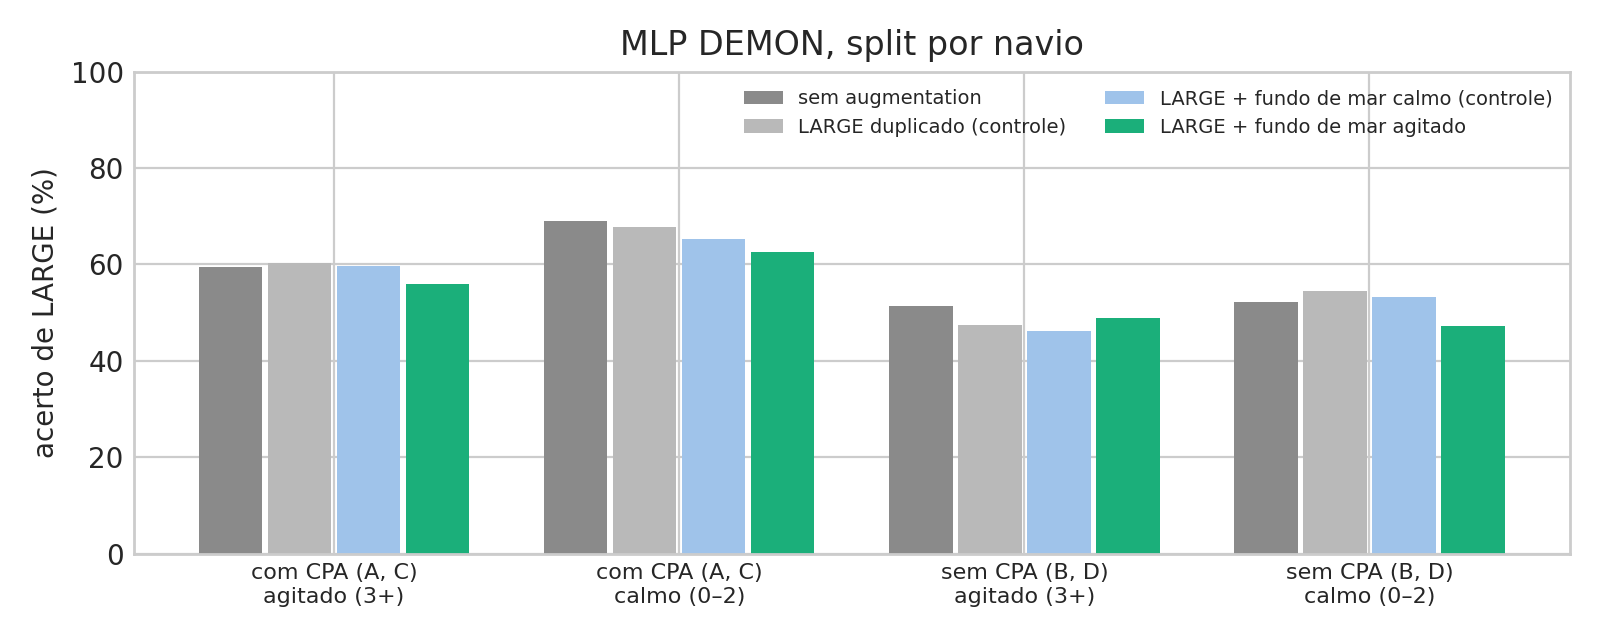
\includegraphics[width=0.8\textwidth]{large_cpa_mar_demon.png}

    \vspace{0.05cm}
    \begin{alertblock}{Leitura}
        \scriptsize
        Onde o efeito era esperado (mar agitado), o acerto cai: com CPA 59 $\rightarrow$ 56\%, sem CPA 51 $\rightarrow$ 49\%. Nenhuma variante melhora nenhum dos quatro grupos de forma consistente.
    \end{alertblock}
\end{frame}

\begin{frame}{LOFAR $\times$ DEMON: Mesmo Resultado}
    \footnotesize
    \begin{table}
    \centering
    \scriptsize
    \setlength{\tabcolsep}{5pt}
    \begin{tabular}{lcccc}
    \toprule
     & \multicolumn{2}{c}{LOFAR} & \multicolumn{2}{c}{DEMON} \\
    \cmidrule(lr){2-3}\cmidrule(lr){4-5}
    Variante & ACC & LARGE & ACC & LARGE \\
    \midrule
    Sem augmentation & 58,3 & 67,7 & 49,4 & 60,8 \\
    dupL (controle) & 58,3 & 67,6 & 47,9 & 60,4 \\
    Fundo calmo (controle) & 57,6 & \calo{63,3} & 48,3 & 58,9 \\
    Fundo agitado & 57,7 & 65,4 & 48,0 & \calo{56,2} \\
    \bottomrule
    \end{tabular}
    \end{table}
    {\tiny Split por navio, mesma MLP, mesmas misturas, 4 classes.\par}
    \vspace{0.1cm}
    \begin{alertblock}{Leitura}
        \scriptsize
        Nas duas representações, misturar fundo tira de 2 a 5 pontos do recall de LARGE e não melhora a acurácia. No LOFAR o fundo calmo prejudicou mais; no DEMON, o agitado. Nenhuma dessas diferenças é significativa.
    \end{alertblock}
\end{frame}

%===========================================
\section{Por Que Não Funciona}

\begin{frame}
    \centering
    \huge Por Que Não Funciona
\end{frame}

\begin{frame}{O Ruído Deixa as Linhas Mais Rasas}
    \centering
    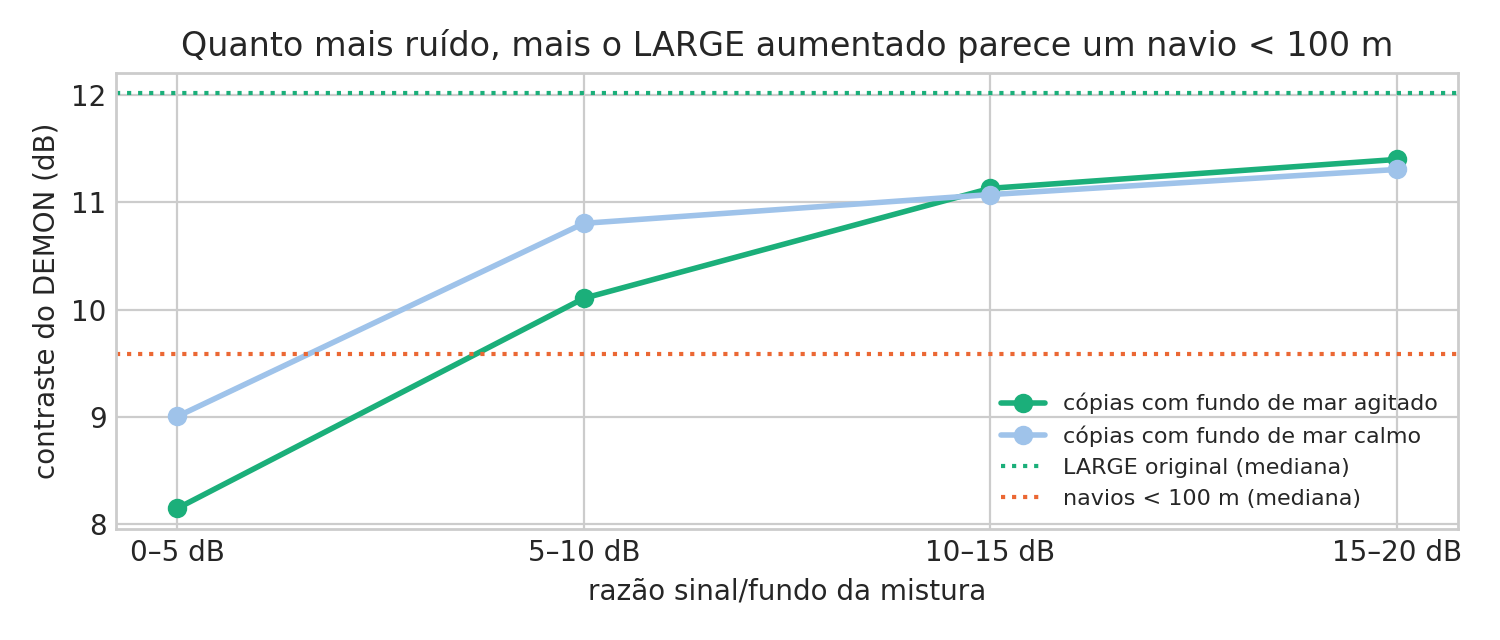
\includegraphics[width=0.74\textwidth]{contraste_rsf.png}

    \vspace{0.05cm}
    \begin{alertblock}{Leitura}
        \scriptsize
        Com mar agitado e muito ruído (0--5 dB), o contraste cai 2,5 dB e \textbf{61\%} das cópias ficam abaixo da mediana dos navios $<$ 100 m (LARGE originais: 28\%). Em todas as razões, 44\% (agitado) e 40\% (calmo). O mar calmo faz quase o mesmo, provavelmente porque a banda de 1--2 kHz recebe bastante ruído mesmo com mar calmo.
    \end{alertblock}
\end{frame}

%===========================================
\section{Conclusões}

\begin{frame}
    \centering
    \huge Conclusões
\end{frame}

\begin{frame}{Conclusões}
    \footnotesize
    \begin{block}{\small O que o DEMON mostra}
        \scriptsize
        \begin{enumerate}
            \setlength{\itemsep}{2pt}
            \item \textbf{O DEMON sozinho é mais fraco que o LOFAR} nas 4 classes (SP 45,7 $\times$ 56,1 no split por navio). Seu papel é complementar o LOFAR ou o MEL.
            \item \textbf{O augmentation com mar agitado não ajuda no DEMON}, assim como não ajudou no LOFAR; repetir os LARGE não muda nada, e misturar qualquer fundo tira um pouco de recall de LARGE.
            \item \textbf{O mecanismo é comum:} o ruído somado ao áudio apaga parte do que identifica o LARGE (o grave no LOFAR, as linhas de modulação no DEMON). O problema está no áudio misturado, não na representação.
        \end{enumerate}
    \end{block}
    \begin{alertblock}{\small Consequência prática}
        \scriptsize
        Mistura com fundo real na faixa de 0--20 dB não é um caminho promissor no IARA. Se for retomada, limitar a razão sinal/fundo (por exemplo, $\geq$ 10 dB) para que a cópia continue sendo um LARGE reconhecível.
    \end{alertblock}
\end{frame}

\end{document}
